\documentclass[../TDE1-E2.tex]{subfiles}%

\begin{document}
\section[s]"2"{Diviseur de tension}

\enonce{%
    \begin{center}
  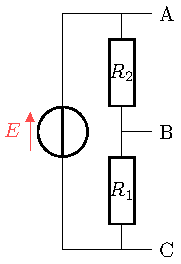
\includegraphics[scale=1, rotate=90]{divtens_plain}
\end{center}
}%

\QR{%
  Écrire la loi des mailles pour le montage ci-contre et en déduire
        l'expression de l'intensité du courant $I(R_2)$ qui parcourt cette
        maille. En déduire l'expression de la tension $U_{BC}$, aux bornes de la
        résistance $R_1$.
}{%
\vspace{-15pt}
\begin{tcbraster}[raster columns=3, raster equal height=rows]
    \begin{tcn}(data){Schéma}
        \begin{center}
            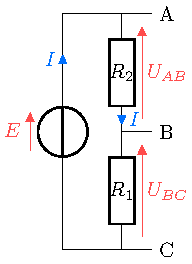
\includegraphics{divtens}
        \end{center}
    \end{tcn}
    \begin{tcolorbox}[blankest, raster multicolumn=1, space to=\myspace]
        \begin{tcbraster}[raster columns=1]
            \begin{tcn}(ques)""{Résultat attendu}
                On cherche $I$ puis $U_{BC}$.
            \end{tcn}
            \begin{tcn}[add to natural height=\myspace](tool)""{Outils}
                \begin{itemize}[leftmargin=10pt]
                    \item Loi des mailles pour $I$~;
                    \item Loi d'Ohm pour $U_{BC}$.
                \end{itemize}
            \end{tcn}
        \end{tcbraster}
    \end{tcolorbox}
    \begin{tcn}(appl)'r'{Application}
        Il suffit d'une loi des mailles pour trouver
        \[I = \frac{E}{R_1+R_2}\]
        Puis trivialement
        \[U_{BC} = R_1I = \frac{R_1}{R_1+R_2}E\]
    \end{tcn}
\end{tcbraster}
\begin{tcbraster}[raster columns=2, raster equal height=rows]
    \begin{tcn}(rema){Remarque}
        On remarque donc que deux dipôles de résistances $R_1$ et $R_2$ se
        partageant une tension totale $E$ vont se la répartir
        en respectant la fraction de résistance à laquelle chaque diôle
        participe. C'est également une simple moyenne pondérée.
    \end{tcn}
    \begin{tcn}(ror)'r'{Important}
        Ce résultat est bien plus général que pour deux dipôles et fonctionne
        avec $n$ dipôles \textbf{\textit{en série}} sur une branche. Il faut
        pouvoir se ramener à ce schéma précis pour appliquer la formule du pont
        diviseur de tension – que vous pouvez maintenant utiliser sans loi des
        mailles~: $\DS U_x = E\times \frac{R_x}{R_\mathrm{tot}}$
    \end{tcn}
\end{tcbraster}
}%

\enonce{%
  On ajoute une résistance $R_3$ qui sera connectée en parallèle avec la
résistance $R_1$.
}%

\QR{%
  Est-ce que la valeur de la tension $U_{BC}$ calculée à la question
        précédente va changer~?
  Si oui, calculer les nouvelles valeurs de $U_{BC}$ et $I(R_2)$.
}{%
\vspace{-15pt}
\begin{tcbraster}[raster columns=3, raster equal height=rows]
    \begin{tcn}(data){Schéma}
        \begin{center}
            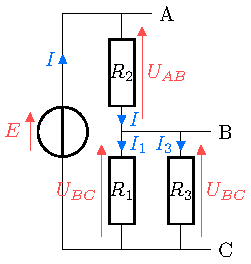
\includegraphics{divtens_b}
        \end{center}
    \end{tcn}
    \begin{tcolorbox}[blankest, raster multicolumn=1, space to=\myspace]
        \begin{tcbraster}[raster columns=1]
            \begin{tcn}(appl)""{Réponse}
                Oui, elle va changer puisqu'on a branché un nouveau dipôle.
            \end{tcn}
            \begin{tcn}(ques)""{Résultat attendu}
                On cherche $I$ et $U_{BC}$.
            \end{tcn}
            \begin{tcn}[add to natural height=\myspace](tool)""{Outils}
                \begin{itemize}[leftmargin=10pt]
                    \item Loi des mailles pour $I$~;
                    \item Loi d'Ohm pour $U_{BC}$.
                \end{itemize}
            \end{tcn}
        \end{tcbraster}
    \end{tcolorbox}
    \begin{tcn}(impl)"limp"'r'{Schéma simplifié}
        \begin{center}
            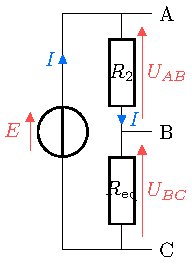
\includegraphics{divtens_b-simple}
        \end{center}
    \end{tcn}
\end{tcbraster}
\begin{center}
    \begin{tcn}[sidebyside](appl){Application}
        On peut envisager ce calcul de deux manières~:
        \begin{itemize}

            \item D'une part, $U_{BC} = R_1 I_1$ et on pourrait déterminer $I_1$
                en fonction de $I$ avec une LdN, et pour ça avoir $I$ avec une
                LdM en calculant $R_{\rm eq}$ comme précédemment, et donc~:

            \item On voit immédiatement que $U_{BC} = R_{\rm eq}I$. Autant
                partir là-dessus.
        \end{itemize}
        \tcblower
        On obtient ainsi \[ R_{\rm eq} = \frac{R_1R_3}{R_1+R_3} \quad \text{et}
        \quad I = \frac{E}{R_2 + \frac{R_1R_3}{R_1+R_3}}\] d'où après calcul
        \[\boxed{U_{BC} = \frac{ER_1R_3}{R_2(R_1+R_3)+R_1R_3}}\]
        %\quad \text{ou}
        %\quad \boxed{U_{BC} = \frac{E}{\frac{R_2}{R_3} + \frac{R_2}{R_1} + 1}}\]
    \end{tcn}
\end{center}
}%

\end{document}
